
\documentclass{article}
\usepackage{fontspec}
\usepackage{xeCJK}
\setmainfont{Times New Roman}
\setCJKmainfont{Hiragino Sans}
\setmonofont{Menlo}
\setCJKmonofont{Hiragino Sans}

\usepackage{amsmath,amssymb,booktabs,longtable,array,calc,graphicx,xcolor,hyperref}
\usepackage[margin=25mm]{geometry}
\hypersetup{colorlinks=true,linkcolor=blue,urlcolor=blue}
\setlength{\parindent}{0pt}
\setlength{\parskip}{6pt}
\providecommand{\tightlist}{\setlength{\itemsep}{0pt}\setlength{\parskip}{0pt}}
\providecommand{\pandocbounded}[1]{\begin{center}\resizebox{0.96\linewidth}{!}{#1}\end{center}}
\newcounter{none}
\makeatletter
\define@key{Gin}{alt}{}
\makeatother

\begin{document}
\section{白猫黒猫灰色猫準安定界面におけるC弱読出しとD強観測選択予備実験総括
v1}\label{ux767dux732bux9ed2ux732bux7070ux8272ux732bux6e96ux5b89ux5b9aux754cux9762ux306bux304aux3051ux308bcux5f31ux8aadux51faux3057ux3068dux5f37ux89b3ux6e2cux9078ux629eux4e88ux5099ux5b9fux9a13ux7dcfux62ec-v1}

\textbf{日付:} 2026-07-14\\
\textbf{著者:} 木原 範昭\\
\textbf{位置づけ:}
波の情報読出しシリーズ・閉鎖系内A/B配分準安定状態と観測選択の予備実験\\
\textbf{Version DOI:} 10.5281/zenodo.21353209\\
\textbf{Concept DOI:} 10.5281/zenodo.21353208

\begin{center}\rule{0.5\linewidth}{0.5pt}\end{center}

\subsection{0. 結論}\label{ux7d50ux8ad6}

本稿は、白猫状態 \texttt{A} と黒猫状態 \texttt{B}
の配分を、閉鎖系内の複素振幅

\[
a,\quad b
\]

として表し、

\[
p_A=|a|^2,\qquad p_B=|b|^2
\]

\[
Q=p_A+p_B,\qquad S=p_A-p_B
\]

を読む予備実験をまとめる。

ここでいう白猫・黒猫・灰色猫は、標準的な猫実験そのものではなく、A/B配分状態を読むための比喩である。

本実験で確認したことは次である。

\begin{verbatim}
1. AB二体だけで、灰色猫固有相、灰色猫準安定相、自然選択相を分離できた。
2. C弱読出しでは、灰色猫準安定相を一方選択せずに読む窓が存在した。
3. D強観測では、灰色猫準安定相が白猫または黒猫へ選択された。
4. 灰色猫固有相では、D強観測を入れても灰色状態が保持された。
5. Dなし対照では白猫・黒猫への同等の落下は起きず、D起因選択として分離できた。
\end{verbatim}

したがって、本実験の結果は次のようにまとめられる。

\begin{verbatim}
灰色猫準安定相:
  弱く読むと灰色として読める。
  強く観測すると白猫または黒猫へ落ちる。

灰色猫固有相:
  弱く読んでも灰色として読める。
  強く観測しても灰色のまま保持される。
\end{verbatim}

白猫に落ちた場合は、

\[
S \simeq +1,\qquad p_A\simeq 1,\qquad p_B\simeq 0
\]

黒猫に落ちた場合は、

\[
S \simeq -1,\qquad p_A\simeq 0,\qquad p_B\simeq 1
\]

である。

これは、白猫と黒猫の二匹へ分岐したというより、A/B配分が片側へほぼ全移動した状態である。

ただし、閉鎖量

\[
Q=p_A+p_B
\]

は保存される。

\begin{center}\rule{0.5\linewidth}{0.5pt}\end{center}

\subsection{1. 背景と目的}\label{ux80ccux666fux3068ux76eeux7684}

波の情報読出しシリーズでは、背景空間を先に置かず、複素位相波の閉鎖関係と干渉読出しから、位置様、運動量様、エネルギー様、加速度様に見える量を構成してきた。

前段の加速度基底・局在性交換実験では、交換干渉散乱行列によるAB相互作用のもとで、局在性と有効倍音次数が相互に再配分される条件を調べた。

本稿では、その流れを、A/B配分状態の選択問題へ移す。

問いは次である。

\begin{verbatim}
白猫Aと黒猫Bが閉鎖系内で混在する状態は、
単なる未選択状態なのか。
それとも、灰色猫固有状態として保持される場合があるのか。

また、弱い読出しCと強い観測Dでは、
その状態はどう変わるのか。
\end{verbatim}

本実験では、この問いを四段階に分ける。

\begin{verbatim}
Stage 1:
  AB二体だけで、灰色猫固有相、灰色猫準安定相、自然選択相を探す。

Stage 2:
  C弱読出しで、灰色猫準安定相を壊さずに読めるか調べる。

Stage 3:
  D強観測で、灰色猫準安定相が白猫または黒猫へ落ちるか調べる。

Stage 4:
  D観測開始ステップとD利得を掃引し、選択境界を読む。
\end{verbatim}

\subsection{1.1 状態遷移図}\label{ux72b6ux614bux9077ux79fbux56f3}

本実験の三つの代表的な読みを、AB、ABC、ABCD
の段階に沿って図示すると次のようになる。

\begin{figure}
\centering
\pandocbounded{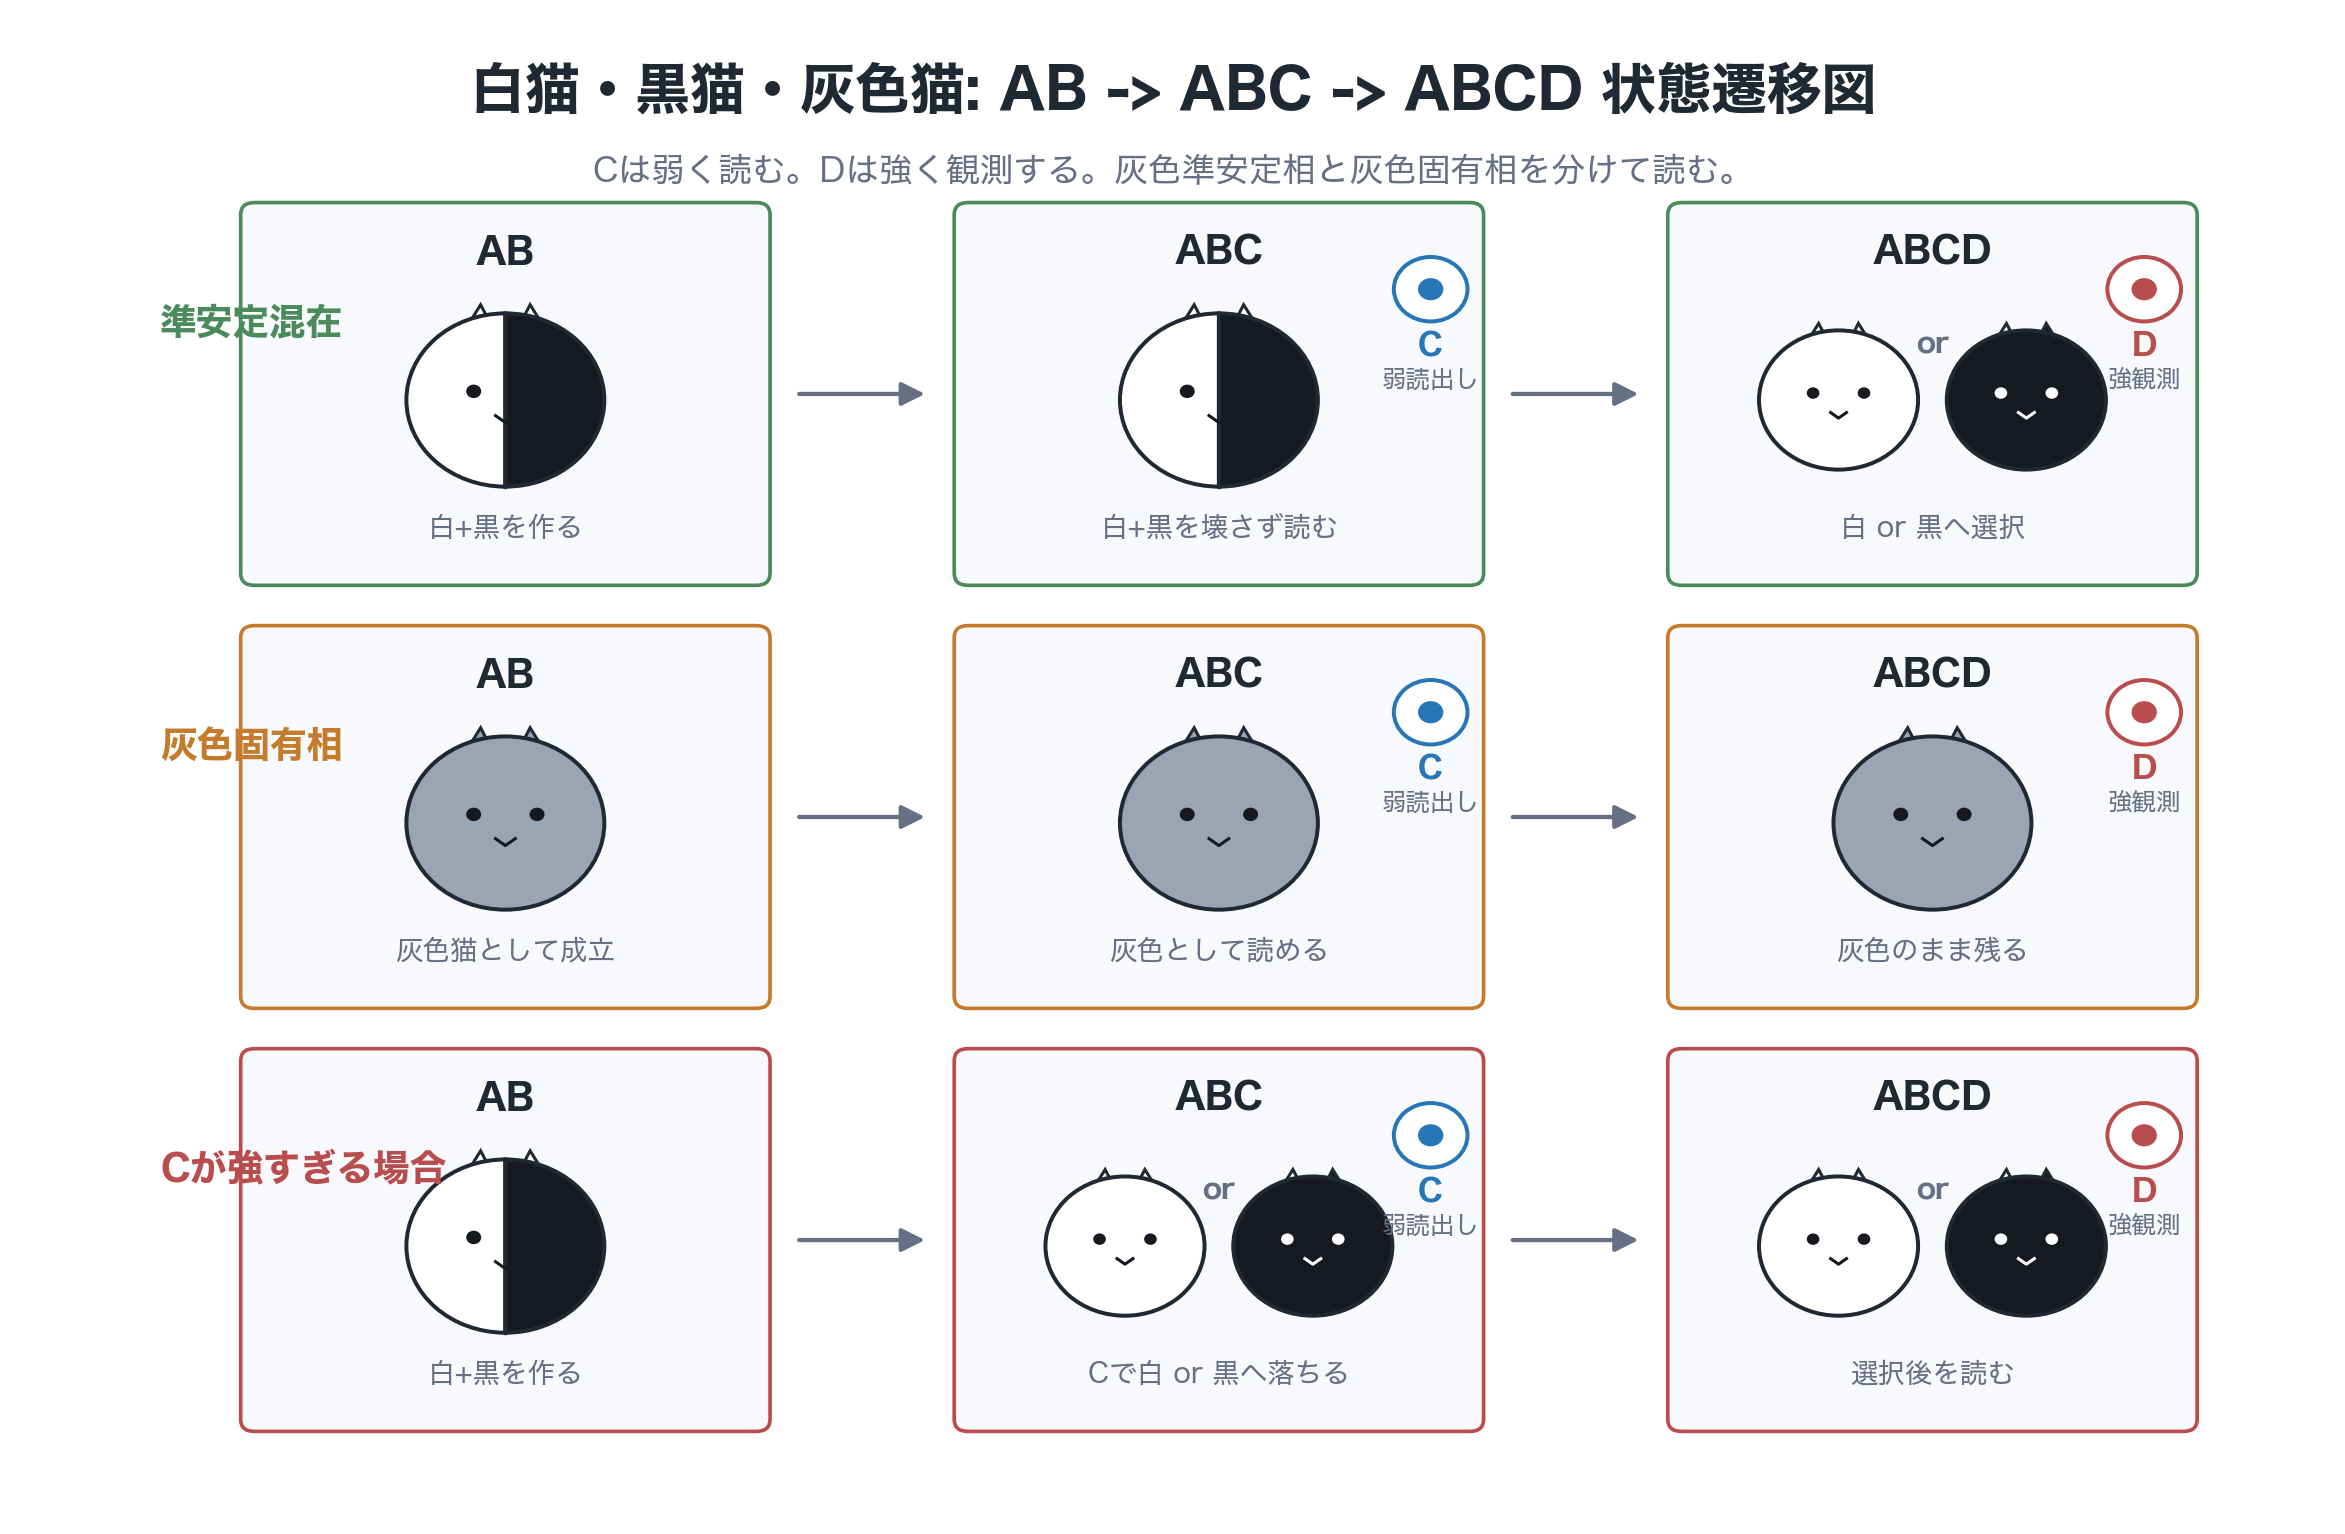
\includegraphics[keepaspectratio,alt={白猫・黒猫・灰色猫 AB-ABC-ABCD 状態遷移図}]{gray_cat_state_transition_figures_v1/gray_cat_ab_abc_abcd_three_scenarios_v1.png}}
\caption{白猫・黒猫・灰色猫 AB-ABC-ABCD 状態遷移図}
\end{figure}

上段は、ABで作った白+黒の準安定混在をCで弱く読み、D強観測で白または黒へ選択する場合である。

中段は、ABの段階で灰色猫固有相になり、C弱読出しでもD強観測でも灰色として保持される場合である。

下段は、Cが強すぎるため、ABCの段階ですでに白または黒への選択が起こる場合である。

\subsection{1.2
実測値による状態遷移図}\label{ux5b9fux6e2cux5024ux306bux3088ux308bux72b6ux614bux9077ux79fbux56f3}

同じ三つの読みを、実際に計算された \texttt{p\_A}, \texttt{p\_B},
\texttt{S} の時系列で図示すると次のようになる。

\begin{figure}
\centering
\pandocbounded{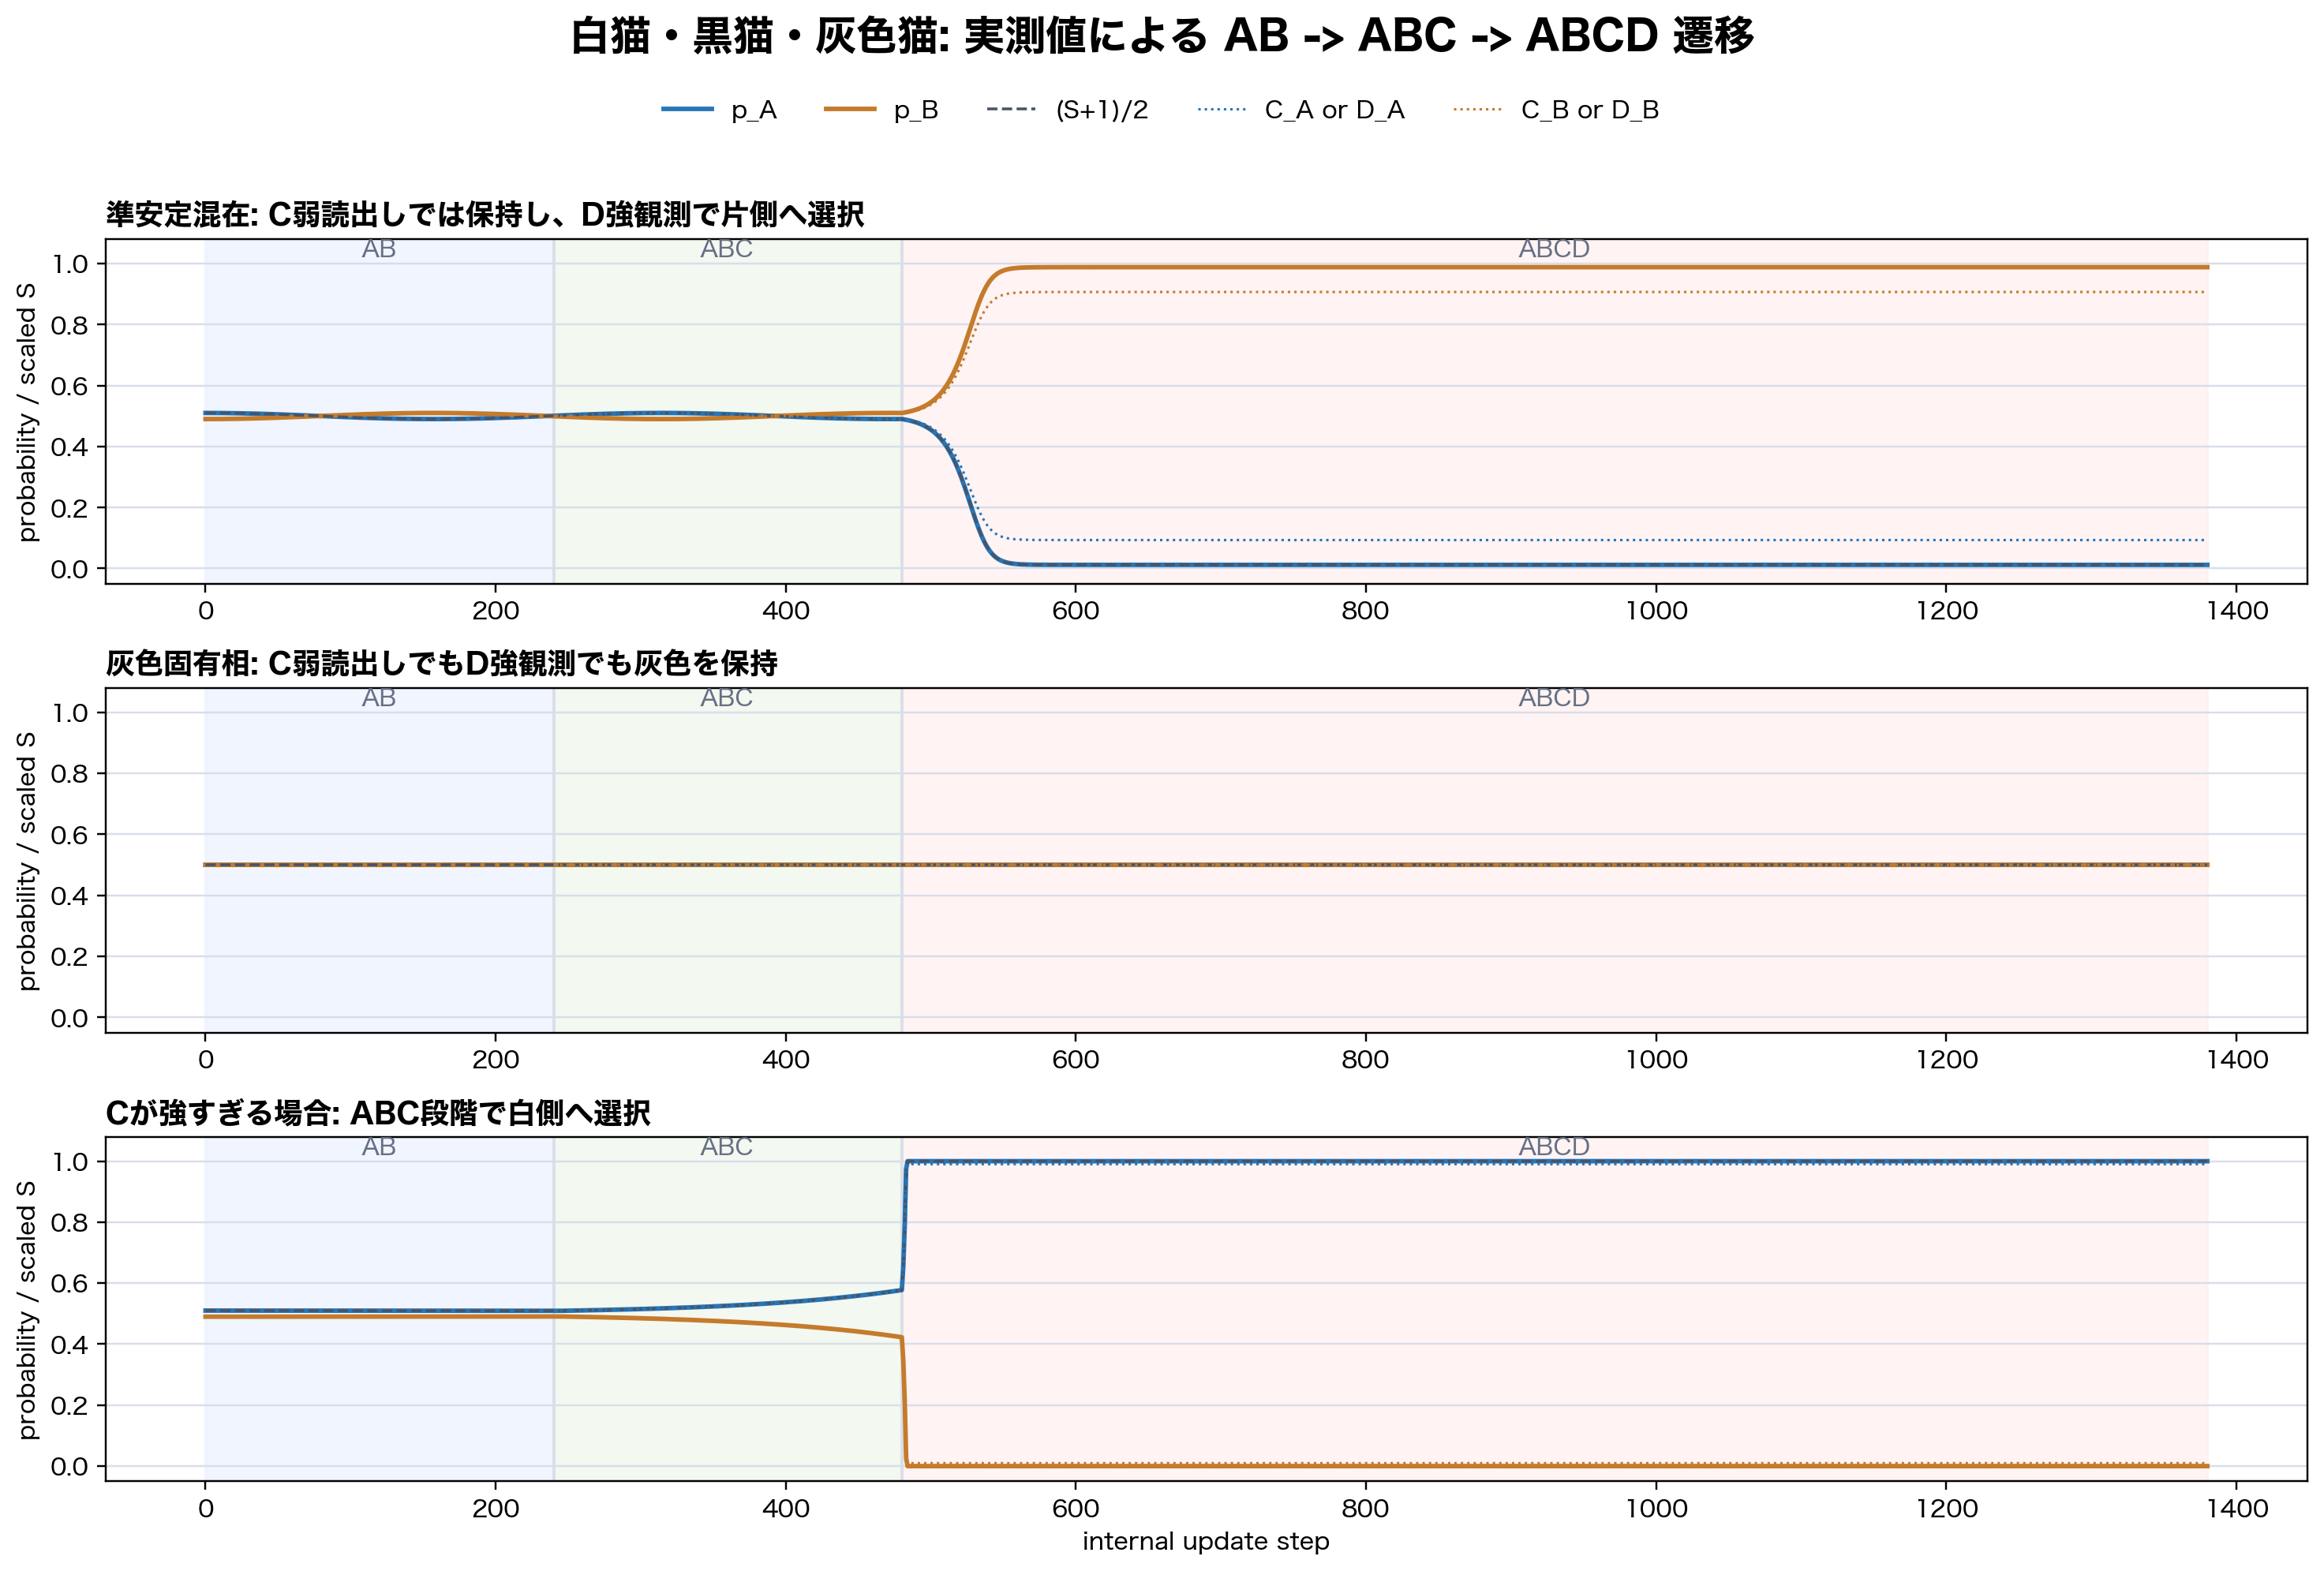
\includegraphics[keepaspectratio,alt={白猫・黒猫・灰色猫 実測値 AB-ABC-ABCD 遷移}]{gray_cat_observed_value_transition_figures_v1/gray_cat_ab_abc_abcd_observed_values_three_scenarios_v1.png}}
\caption{白猫・黒猫・灰色猫 実測値 AB-ABC-ABCD 遷移}
\end{figure}

実線は内部状態の \texttt{p\_A}, \texttt{p\_B} である。

破線は、比較のために

\[
\frac{S+1}{2}
\]

として同じ縦軸へ写した選択秩序変数である。

点線は、ABC区間ではC読出し、ABCD区間ではD読出しを示す。

この図では、準安定混在、灰色固有相、Cが強すぎる場合の三者が、同じ
\texttt{p\_A,p\_B,S} の読出し上で分離している。

\begin{center}\rule{0.5\linewidth}{0.5pt}\end{center}

\subsection{2. 変数と相分類}\label{ux5909ux6570ux3068ux76f8ux5206ux985e}

\subsection{2.1 A/B配分}\label{abux914dux5206}

A/B配分は、

\[
p_A=|a|^2,\qquad p_B=|b|^2
\]

で読む。

閉鎖量は、

\[
Q=p_A+p_B
\]

である。

A/B選択秩序変数を、

\[
S=p_A-p_B
\]

とする。

このとき、

\[
p_A=\frac{1+S}{2},
\qquad
p_B=\frac{1-S}{2}
\]

である。

\subsection{2.2
白猫・黒猫・灰色猫}\label{ux767dux732bux9ed2ux732bux7070ux8272ux732b}

本稿では、次の読替えを用いる。

{\def\LTcaptype{none} % do not increment counter
\begin{longtable}[]{@{}lll@{}}
\toprule\noalign{}
状態 & 数値条件の目安 & 読み \\
\midrule\noalign{}
\endhead
\bottomrule\noalign{}
\endlastfoot
白猫 & \texttt{S≈+1} & \texttt{p\_A≈1}, \texttt{p\_B≈0} \\
黒猫 & \texttt{S≈-1} & \texttt{p\_A≈0}, \texttt{p\_B≈1} \\
灰色猫 & \texttt{S≈0} & \texttt{p\_A≈0.5}, \texttt{p\_B≈0.5} \\
\end{longtable}
}

\subsection{2.3 相分類}\label{ux76f8ux5206ux985e}

AB二体だけの発展では、次の相を分類する。

\begin{verbatim}
gray_eigen:
  S_mean ≈ 0
  S_amp ≈ 0
  S_drift ≈ 0

gray_metastable:
  S_mean ≈ 0
  0 < S_amp < S_gray_limit
  S_drift ≈ 0

natural_selection:
  CもDもないのに S -> +1 または S -> -1 へ落ちる。

large_oscillation:
  Sが大きく振動し、A/B偏りが明確に現れる。
\end{verbatim}

本稿の中心対象は \texttt{gray\_metastable} と \texttt{gray\_eigen}
である。

\begin{center}\rule{0.5\linewidth}{0.5pt}\end{center}

\subsection{3. モデル}\label{ux30e2ux30c7ux30eb}

\subsection{3.1
AB交換相互作用}\label{abux4ea4ux63dbux76f8ux4e92ux4f5cux7528}

AB二体の最小交換写像は、

\[
\begin{pmatrix}
a_{k+1}\\
b_{k+1}
\end{pmatrix}
=
U_\epsilon
\begin{pmatrix}
a_k\\
b_k
\end{pmatrix}
\]

\[
U_\epsilon
=
\begin{pmatrix}
\cos\epsilon & i\sin\epsilon\\
i\sin\epsilon & \cos\epsilon
\end{pmatrix}
\]

である。

必要に応じて、閉鎖系内の安定性を調べるため、弱い復元項または弱い非線形項を加える。

ただし、Cなし・Dなしで自然選択する条件は、観測による選択の候補から除外する。

\subsection{3.2 C弱読出し}\label{cux5f31ux8aadux51faux3057}

Cは、A/B配分を弱く読む内部読出し波である。

可視度を、

\[
v_C=\frac{g_C}{g_C+\kappa_C}
\]

とし、

\[
S_C=v_CS
\]

\[
C_A=\frac{1+S_C}{2},
\qquad
C_B=\frac{1-S_C}{2}
\]

として読む。

Cは、A/B配分を読むが、一方選択を起こさない窓を探すために用いる。

\subsection{3.3 D強観測}\label{dux5f37ux89b3ux6e2c}

Dは、現在の \texttt{S} を読んだ方向へ増幅する強観測写像である。

可視度を、

\[
v_D=\frac{g_D}{g_D+\kappa_D}
\]

とし、

\[
S_D=v_DS
\]

を読む。

Dバックアクションは、

\[
S_{k+1}
=
S_k
+
G_D S_D(1-S_k^2)
\]

として実装する。

ここで \texttt{G\_D} はD利得である。

同じD開始状態からDなし対照を並走させ、Dなし対照でも同じ白猫または黒猫選択が起こる場合は、D起因選択とは数えない。

\begin{center}\rule{0.5\linewidth}{0.5pt}\end{center}

\subsection{4. Stage 1:
AB準安定界面探索}\label{stage-1-abux6e96ux5b89ux5b9aux754cux9762ux63a2ux7d22}

\subsection{4.1 条件}\label{ux6761ux4ef6}

\begin{verbatim}
C = off
D = off
steps = 4096
S_gray_limit = 0.05
selection_limit = 0.95
\end{verbatim}

掃引した主なパラメータは次である。

\begin{verbatim}
epsilon_values = (0.0, 1e-05, 3e-05, 0.0001, 0.0003, 0.001, 0.003, 0.01)
stability_gain_values = (-0.01, -0.002, 0.0, 0.002, 0.01)
\end{verbatim}

\subsection{4.2 結果}\label{ux7d50ux679c}

{\def\LTcaptype{none} % do not increment counter
\begin{longtable}[]{@{}lr@{}}
\toprule\noalign{}
phase & count \\
\midrule\noalign{}
\endhead
\bottomrule\noalign{}
\endlastfoot
\texttt{gray\_eigen} & \texttt{1248} \\
\texttt{gray\_metastable} & \texttt{733} \\
\texttt{large\_oscillation} & \texttt{470} \\
\texttt{natural\_selection} & \texttt{1070} \\
\texttt{unstable\_or\_drifting} & \texttt{2079} \\
\end{longtable}
}

AB二体だけで、灰色猫固有相、灰色猫準安定相、大振幅振動領域、自然選択相が分離して観測された。

代表的な灰色猫準安定候補は次である。

{\def\LTcaptype{none} % do not increment counter
\begin{longtable}[]{@{}
  >{\raggedleft\arraybackslash}p{(\linewidth - 12\tabcolsep) * \real{0.1429}}
  >{\raggedleft\arraybackslash}p{(\linewidth - 12\tabcolsep) * \real{0.1429}}
  >{\raggedleft\arraybackslash}p{(\linewidth - 12\tabcolsep) * \real{0.1429}}
  >{\raggedleft\arraybackslash}p{(\linewidth - 12\tabcolsep) * \real{0.1429}}
  >{\raggedleft\arraybackslash}p{(\linewidth - 12\tabcolsep) * \real{0.1429}}
  >{\raggedleft\arraybackslash}p{(\linewidth - 12\tabcolsep) * \real{0.1429}}
  >{\raggedleft\arraybackslash}p{(\linewidth - 12\tabcolsep) * \real{0.1429}}@{}}
\toprule\noalign{}
\begin{minipage}[b]{\linewidth}\raggedleft
epsilon
\end{minipage} & \begin{minipage}[b]{\linewidth}\raggedleft
phi/pi
\end{minipage} & \begin{minipage}[b]{\linewidth}\raggedleft
s0
\end{minipage} & \begin{minipage}[b]{\linewidth}\raggedleft
gain
\end{minipage} & \begin{minipage}[b]{\linewidth}\raggedleft
S\_mean
\end{minipage} & \begin{minipage}[b]{\linewidth}\raggedleft
S\_amp
\end{minipage} & \begin{minipage}[b]{\linewidth}\raggedleft
S\_drift
\end{minipage} \\
\midrule\noalign{}
\endhead
\bottomrule\noalign{}
\endlastfoot
\texttt{0.01} & \texttt{0} & \texttt{0.01} & \texttt{0} &
\texttt{0.000173315} & \texttt{0.02} & \texttt{0.00205793} \\
\texttt{0.01} & \texttt{1} & \texttt{0.01} & \texttt{0} &
\texttt{0.000173315} & \texttt{0.02} & \texttt{0.00205793} \\
\texttt{0.003} & \texttt{0.0833333} & \texttt{0} & \texttt{-0.002} &
\texttt{-0.00213507} & \texttt{0.020193} & \texttt{0.00227521} \\
\end{longtable}
}

\begin{center}\rule{0.5\linewidth}{0.5pt}\end{center}

\subsection{5. Stage 2:
C弱読出し窓}\label{stage-2-cux5f31ux8aadux51faux3057ux7a93}

\subsection{5.1 条件}\label{ux6761ux4ef6-1}

\begin{verbatim}
C = on
D = off
steps = 4096
readout_kappa = 0.02
g_C_values = (0.0, 0.002, 0.005, 0.01, 0.02, 0.05, 0.1, 0.2, 0.5, 1.0)
backaction_scale_values = (0.0, 1e-05, 5e-05, 0.0001, 0.0005, 0.001, 0.002, 0.005, 0.01)
\end{verbatim}

\subsection{5.2 結果}\label{ux7d50ux679c-1}

\begin{verbatim}
total_cases = 1080
C_window_count = 247
C_informative_window_count = 144
C_nonzero_backaction_window_count = 114
\end{verbatim}

C後の相分類は次であった。

{\def\LTcaptype{none} % do not increment counter
\begin{longtable}[]{@{}lr@{}}
\toprule\noalign{}
phase\_after\_C & count \\
\midrule\noalign{}
\endhead
\bottomrule\noalign{}
\endlastfoot
\texttt{gray\_eigen} & \texttt{90} \\
\texttt{gray\_metastable} & \texttt{786} \\
\texttt{large\_oscillation} & \texttt{141} \\
\texttt{natural\_selection} & \texttt{2} \\
\texttt{unstable\_or\_drifting} & \texttt{61} \\
\end{longtable}
}

灰色猫準安定候補にCを加え、A/B配分を読めるが一方選択を起こさない結合窓を確認した。

非ゼロCバックアクションを持つ代表的読出し窓は次である。

{\def\LTcaptype{none} % do not increment counter
\begin{longtable}[]{@{}
  >{\raggedleft\arraybackslash}p{(\linewidth - 16\tabcolsep) * \real{0.1143}}
  >{\raggedleft\arraybackslash}p{(\linewidth - 16\tabcolsep) * \real{0.1143}}
  >{\raggedleft\arraybackslash}p{(\linewidth - 16\tabcolsep) * \real{0.1143}}
  >{\raggedleft\arraybackslash}p{(\linewidth - 16\tabcolsep) * \real{0.1143}}
  >{\raggedleft\arraybackslash}p{(\linewidth - 16\tabcolsep) * \real{0.1143}}
  >{\raggedleft\arraybackslash}p{(\linewidth - 16\tabcolsep) * \real{0.1143}}
  >{\raggedleft\arraybackslash}p{(\linewidth - 16\tabcolsep) * \real{0.1143}}
  >{\raggedleft\arraybackslash}p{(\linewidth - 16\tabcolsep) * \real{0.1143}}
  >{\raggedright\arraybackslash}p{(\linewidth - 16\tabcolsep) * \real{0.0857}}@{}}
\toprule\noalign{}
\begin{minipage}[b]{\linewidth}\raggedleft
epsilon
\end{minipage} & \begin{minipage}[b]{\linewidth}\raggedleft
phi/pi
\end{minipage} & \begin{minipage}[b]{\linewidth}\raggedleft
s0
\end{minipage} & \begin{minipage}[b]{\linewidth}\raggedleft
base\_gain
\end{minipage} & \begin{minipage}[b]{\linewidth}\raggedleft
g\_C
\end{minipage} & \begin{minipage}[b]{\linewidth}\raggedleft
c\_gain
\end{minipage} & \begin{minipage}[b]{\linewidth}\raggedleft
C\_rel\_err
\end{minipage} & \begin{minipage}[b]{\linewidth}\raggedleft
C\_bias\_delta
\end{minipage} & \begin{minipage}[b]{\linewidth}\raggedright
phase\_after\_C
\end{minipage} \\
\midrule\noalign{}
\endhead
\bottomrule\noalign{}
\endlastfoot
\texttt{0.003} & \texttt{0.0833333} & \texttt{0} & \texttt{-0.002} &
\texttt{1} & \texttt{5e-05} & \texttt{0.0196078} & \texttt{0.00122196} &
\texttt{gray\_metastable} \\
\texttt{0.003} & \texttt{0.0833333} & \texttt{0} & \texttt{-0.002} &
\texttt{1} & \texttt{1e-05} & \texttt{0.0196078} & \texttt{0.000220996}
& \texttt{gray\_metastable} \\
\texttt{0.003} & \texttt{0.0833333} & \texttt{0.001} & \texttt{-0.002} &
\texttt{1} & \texttt{1e-05} & \texttt{0.0196078} & \texttt{0.000222243}
& \texttt{gray\_metastable} \\
\end{longtable}
}

\begin{center}\rule{0.5\linewidth}{0.5pt}\end{center}

\subsection{6. Stage 3:
D強観測応答}\label{stage-3-dux5f37ux89b3ux6e2cux5fdcux7b54}

\subsection{6.1 条件}\label{ux6761ux4ef6-2}

\begin{verbatim}
Stage 1: AB準安定界面探索済み
Stage 2: C読出し窓確認済み
Stage 3: D強観測応答
pre_steps_values = (0, 1, 2, 5, 10, 20, 50, 100, 250, 500, 1000, 2000)
d_steps = 2048
c_modes = (record_only, weak_C_window)
g_D_values = (0.0, 0.05, 0.1, 0.2, 0.5, 1.0)
d_backaction_scale_values = (0.0, 0.02, 0.05, 0.1, 0.2, 0.5, 1.0)
\end{verbatim}

\subsection{6.2 全体結果}\label{ux5168ux4f53ux7d50ux679c}

\begin{verbatim}
total_cases = 7056
D_induced_selection_count = 2016
\end{verbatim}

D結果分類は次である。

{\def\LTcaptype{none} % do not increment counter
\begin{longtable}[]{@{}lr@{}}
\toprule\noalign{}
D\_outcome & count \\
\midrule\noalign{}
\endhead
\bottomrule\noalign{}
\endlastfoot
\texttt{white\_selected} & \texttt{1244} \\
\texttt{black\_selected} & \texttt{772} \\
\texttt{gray\_kept\_eigen} & \texttt{1062} \\
\texttt{unresolved} & \texttt{3978} \\
\end{longtable}
}

Dなし対照では、次であった。

{\def\LTcaptype{none} % do not increment counter
\begin{longtable}[]{@{}lr@{}}
\toprule\noalign{}
baseline\_outcome & count \\
\midrule\noalign{}
\endhead
\bottomrule\noalign{}
\endlastfoot
\texttt{gray\_kept\_eigen} & \texttt{1176} \\
\texttt{unresolved} & \texttt{5880} \\
\end{longtable}
}

Dなし対照では、白猫または黒猫への同等の落下は検出されなかった。

\subsection{6.3
灰色猫固有相}\label{ux7070ux8272ux732bux56faux6709ux76f8}

灰色猫固有相では、強D条件でも次が確認された。

{\def\LTcaptype{none} % do not increment counter
\begin{longtable}[]{@{}
  >{\raggedleft\arraybackslash}p{(\linewidth - 12\tabcolsep) * \real{0.1538}}
  >{\raggedright\arraybackslash}p{(\linewidth - 12\tabcolsep) * \real{0.1154}}
  >{\raggedleft\arraybackslash}p{(\linewidth - 12\tabcolsep) * \real{0.1538}}
  >{\raggedright\arraybackslash}p{(\linewidth - 12\tabcolsep) * \real{0.1154}}
  >{\raggedleft\arraybackslash}p{(\linewidth - 12\tabcolsep) * \real{0.1538}}
  >{\raggedleft\arraybackslash}p{(\linewidth - 12\tabcolsep) * \real{0.1538}}
  >{\raggedleft\arraybackslash}p{(\linewidth - 12\tabcolsep) * \real{0.1538}}@{}}
\toprule\noalign{}
\begin{minipage}[b]{\linewidth}\raggedleft
pre
\end{minipage} & \begin{minipage}[b]{\linewidth}\raggedright
C\_mode
\end{minipage} & \begin{minipage}[b]{\linewidth}\raggedleft
S\_start
\end{minipage} & \begin{minipage}[b]{\linewidth}\raggedright
outcome
\end{minipage} & \begin{minipage}[b]{\linewidth}\raggedleft
S\_mean\_after\_D
\end{minipage} & \begin{minipage}[b]{\linewidth}\raggedleft
S\_amp\_after\_D
\end{minipage} & \begin{minipage}[b]{\linewidth}\raggedleft
Q\_err
\end{minipage} \\
\midrule\noalign{}
\endhead
\bottomrule\noalign{}
\endlastfoot
\texttt{0} & \texttt{record\_only} & \texttt{0} &
\texttt{gray\_kept\_eigen} & \texttt{0} & \texttt{0} &
\texttt{2.22e-16} \\
\texttt{0} & \texttt{weak\_C\_window} & \texttt{0} &
\texttt{gray\_kept\_eigen} & \texttt{0} & \texttt{0} &
\texttt{2.22e-16} \\
\texttt{20} & \texttt{record\_only} & \texttt{0} &
\texttt{gray\_kept\_eigen} & \texttt{0} & \texttt{0} &
\texttt{2.22e-16} \\
\texttt{20} & \texttt{weak\_C\_window} & \texttt{0} &
\texttt{gray\_kept\_eigen} & \texttt{0} & \texttt{0} &
\texttt{2.22e-16} \\
\end{longtable}
}

灰色猫固有相は、D強観測によって白猫または黒猫へ落ちなかった。

\subsection{6.4
灰色猫準安定相}\label{ux7070ux8272ux732bux6e96ux5b89ux5b9aux76f8}

灰色猫準安定相では、D強観測により白猫または黒猫への選択が起きた。

代表例は次である。

{\def\LTcaptype{none} % do not increment counter
\begin{longtable}[]{@{}
  >{\raggedleft\arraybackslash}p{(\linewidth - 20\tabcolsep) * \real{0.0952}}
  >{\raggedleft\arraybackslash}p{(\linewidth - 20\tabcolsep) * \real{0.0952}}
  >{\raggedleft\arraybackslash}p{(\linewidth - 20\tabcolsep) * \real{0.0952}}
  >{\raggedleft\arraybackslash}p{(\linewidth - 20\tabcolsep) * \real{0.0952}}
  >{\raggedleft\arraybackslash}p{(\linewidth - 20\tabcolsep) * \real{0.0952}}
  >{\raggedleft\arraybackslash}p{(\linewidth - 20\tabcolsep) * \real{0.0952}}
  >{\raggedleft\arraybackslash}p{(\linewidth - 20\tabcolsep) * \real{0.0952}}
  >{\raggedleft\arraybackslash}p{(\linewidth - 20\tabcolsep) * \real{0.0952}}
  >{\raggedright\arraybackslash}p{(\linewidth - 20\tabcolsep) * \real{0.0714}}
  >{\raggedright\arraybackslash}p{(\linewidth - 20\tabcolsep) * \real{0.0714}}
  >{\raggedleft\arraybackslash}p{(\linewidth - 20\tabcolsep) * \real{0.0952}}@{}}
\toprule\noalign{}
\begin{minipage}[b]{\linewidth}\raggedleft
epsilon
\end{minipage} & \begin{minipage}[b]{\linewidth}\raggedleft
phi/pi
\end{minipage} & \begin{minipage}[b]{\linewidth}\raggedleft
s0
\end{minipage} & \begin{minipage}[b]{\linewidth}\raggedleft
gain
\end{minipage} & \begin{minipage}[b]{\linewidth}\raggedleft
pre
\end{minipage} & \begin{minipage}[b]{\linewidth}\raggedleft
S\_start
\end{minipage} & \begin{minipage}[b]{\linewidth}\raggedleft
g\_D
\end{minipage} & \begin{minipage}[b]{\linewidth}\raggedleft
D\_gain
\end{minipage} & \begin{minipage}[b]{\linewidth}\raggedright
outcome
\end{minipage} & \begin{minipage}[b]{\linewidth}\raggedright
baseline
\end{minipage} & \begin{minipage}[b]{\linewidth}\raggedleft
S\_mean\_after\_D
\end{minipage} \\
\midrule\noalign{}
\endhead
\bottomrule\noalign{}
\endlastfoot
\texttt{0.003} & \texttt{0.0833333} & \texttt{0} & \texttt{-0.002} &
\texttt{0} & \texttt{0} & \texttt{1} & \texttt{1} &
\texttt{black\_selected} & \texttt{unresolved} & \texttt{-1} \\
\texttt{0.003} & \texttt{0.0833333} & \texttt{0} & \texttt{-0.002} &
\texttt{0} & \texttt{0} & \texttt{0.5} & \texttt{0.25} &
\texttt{black\_selected} & \texttt{unresolved} & \texttt{-0.999878} \\
\texttt{0.01} & \texttt{0} & \texttt{0.01} & \texttt{0} & \texttt{0} &
\texttt{0.02} & \texttt{1} & \texttt{0.2} & \texttt{white\_selected} &
\texttt{unresolved} & \texttt{0.997467} \\
\end{longtable}
}

\subsection{6.5
大振幅分離領域}\label{ux5927ux632fux5e45ux5206ux96e2ux9818ux57df}

大振幅分離領域では、D結果がC読出し符号と一致する条件を確認した。

{\def\LTcaptype{none} % do not increment counter
\begin{longtable}[]{@{}rrllrl@{}}
\toprule\noalign{}
pre & S\_start & C\_sign & outcome & S\_mean\_after\_D & agreement \\
\midrule\noalign{}
\endhead
\bottomrule\noalign{}
\endlastfoot
\texttt{0} & \texttt{0.06} & \texttt{A} & \texttt{white\_selected} &
\texttt{1} & \texttt{same\_sign} \\
\texttt{1} & \texttt{0.0556528} & \texttt{A} & \texttt{white\_selected}
& \texttt{1} & \texttt{same\_sign} \\
\texttt{2} & \texttt{0.0513121} & \texttt{A} & \texttt{white\_selected}
& \texttt{1} & \texttt{same\_sign} \\
\end{longtable}
}

この領域では、Dが新たに選択を作ったというより、すでに系内に現れたA/B偏りを強く読んだものとして扱う。

\begin{center}\rule{0.5\linewidth}{0.5pt}\end{center}

\subsection{7. Stage 4:
D選択境界}\label{stage-4-dux9078ux629eux5883ux754c}

\subsection{7.1 条件}\label{ux6761ux4ef6-3}

対象は、Stage 3でD起因選択が確認された灰色猫準安定候補である。

\begin{verbatim}
target = gray_metastable candidates only
d_steps = 2048
pre_steps_values_count = 73
C_modes = (record_only, weak_C_window)
\end{verbatim}

D利得は、境界近傍を細かく刻んだ。

\begin{verbatim}
D_gain_values =
(0.0, 0.005, 0.01, 0.015, 0.02,
 0.0225, 0.025, 0.0275, 0.03,
 0.0325, 0.035, 0.0375, 0.04,
 0.045, 0.05, 0.055, 0.06,
 0.065, 0.07, 0.0725, 0.075,
 0.0775, 0.08, 0.0825, 0.085,
 0.0875, 0.09, 0.095, 0.1,
 0.12, 0.15, 0.2, 0.3,
 0.5, 0.75, 1.0)
\end{verbatim}

\subsection{7.2 結果}\label{ux7d50ux679c-2}

\begin{verbatim}
total_rows = 15768
boundary_points = 438
selection_possible_boundary_points = 438
no_selection_boundary_points = 0
min_D_gain_overall = 0.0225
max_min_D_gain_overall = 0.065
\end{verbatim}

候補別の境界は次である。

{\def\LTcaptype{none} % do not increment counter
\begin{longtable}[]{@{}
  >{\raggedright\arraybackslash}p{(\linewidth - 12\tabcolsep) * \real{0.1154}}
  >{\raggedleft\arraybackslash}p{(\linewidth - 12\tabcolsep) * \real{0.1538}}
  >{\raggedleft\arraybackslash}p{(\linewidth - 12\tabcolsep) * \real{0.1538}}
  >{\raggedleft\arraybackslash}p{(\linewidth - 12\tabcolsep) * \real{0.1538}}
  >{\raggedleft\arraybackslash}p{(\linewidth - 12\tabcolsep) * \real{0.1538}}
  >{\raggedleft\arraybackslash}p{(\linewidth - 12\tabcolsep) * \real{0.1538}}
  >{\raggedright\arraybackslash}p{(\linewidth - 12\tabcolsep) * \real{0.1154}}@{}}
\toprule\noalign{}
\begin{minipage}[b]{\linewidth}\raggedright
case\_id
\end{minipage} & \begin{minipage}[b]{\linewidth}\raggedleft
boundary\_points
\end{minipage} & \begin{minipage}[b]{\linewidth}\raggedleft
selection\_possible
\end{minipage} & \begin{minipage}[b]{\linewidth}\raggedleft
no\_selection
\end{minipage} & \begin{minipage}[b]{\linewidth}\raggedleft
min\_gain
\end{minipage} & \begin{minipage}[b]{\linewidth}\raggedleft
max\_min\_gain
\end{minipage} & \begin{minipage}[b]{\linewidth}\raggedright
sign\_counts
\end{minipage} \\
\midrule\noalign{}
\endhead
\bottomrule\noalign{}
\endlastfoot
\texttt{gray\_metastable\_0\_eps0.01\_phi0\_s0.01\_g0} & \texttt{146} &
\texttt{146} & \texttt{0} & \texttt{0.065} & \texttt{0.065} &
\texttt{A:90,\ B:56} \\
\texttt{gray\_metastable\_1\_eps0.01\_phi1\_s0.01\_g0} & \texttt{146} &
\texttt{146} & \texttt{0} & \texttt{0.065} & \texttt{0.065} &
\texttt{A:90,\ B:56} \\
\texttt{gray\_metastable\_4\_eps0.003\_phi0.0833333\_s0\_g-0.002} &
\texttt{146} & \texttt{146} & \texttt{0} & \texttt{0.0225} &
\texttt{0.0225} & \texttt{B:114,\ A:32} \\
\end{longtable}
}

今回の掃引範囲では、対象とした全ての観測開始ステップでD起因選択が可能であった。

候補ごとの最小D利得は二段に分かれた。

\begin{verbatim}
weak threshold candidate:
  min_D_gain = 0.0225

strong threshold candidates:
  min_D_gain = 0.065
\end{verbatim}

\begin{center}\rule{0.5\linewidth}{0.5pt}\end{center}

\subsection{8. 考察}\label{ux8003ux5bdf}

本実験で重要なのは、灰色猫が一種類ではなかったことである。

灰色猫準安定相は、弱く読めば灰色として読める。

しかし、強いD観測を入れると、白猫または黒猫へ落ちる。

このとき、白猫になれば

\[
p_A\simeq 1,\qquad p_B\simeq 0
\]

黒猫になれば

\[
p_A\simeq 0,\qquad p_B\simeq 1
\]

である。

したがって、白猫と黒猫が二匹同時に出るのではない。

A/B配分が片側へ移り、反対側の成分は読出し上ほぼ消える。

一方、灰色猫固有相では、強いD観測を入れても

\[
p_A\simeq 0.5,\qquad p_B\simeq 0.5
\]

が保持された。

これは、灰色猫準安定相と灰色猫固有相を、観測応答で区別できることを示す。

また、C弱読出しでは、選択を起こさずにA/B配分を読む窓があった。

したがって、本実験では、次の三つが分離された。

\begin{verbatim}
AB二体だけで自然に落ちる自然選択。
C弱読出しで壊さず読める準安定灰色状態。
D強観測で白猫または黒猫へ落ちる選択状態。
\end{verbatim}

\begin{center}\rule{0.5\linewidth}{0.5pt}\end{center}

\subsection{9. 結論}\label{ux7d50ux8ad6-1}

本実験により、閉鎖系内のA/B配分状態について、次を確認した。

\begin{verbatim}
1. AB交換相互作用だけで、灰色猫固有相、灰色猫準安定相、自然選択相を分類できる。
2. C弱読出しには、灰色猫準安定相を選択せずに読む窓がある。
3. D強観測では、灰色猫準安定相が白猫または黒猫へ落ちる。
4. 灰色猫固有相は、D強観測でも灰色状態を保持する。
5. D選択境界では、対象とした全ての準安定候補でD起因選択が可能だった。
6. 最小D利得は、候補によって 0.0225 と 0.065 の二段に分かれた。
\end{verbatim}

したがって、白猫・黒猫・灰色猫という三状態は、単一の未選択状態ではなく、閉鎖系内の相分類と観測強度によって分かれる。

特に、

\begin{verbatim}
灰色猫準安定相:
  弱読出しでは灰色。
  強観測では白または黒。

灰色猫固有相:
  強観測でも灰色。
\end{verbatim}

という分岐を得た。

\begin{center}\rule{0.5\linewidth}{0.5pt}\end{center}

\subsection{10. 出力}\label{ux51faux529b}

{\def\LTcaptype{none} % do not increment counter
\begin{longtable}[]{@{}
  >{\raggedright\arraybackslash}p{(\linewidth - 2\tabcolsep) * \real{0.5000}}
  >{\raggedright\arraybackslash}p{(\linewidth - 2\tabcolsep) * \real{0.5000}}@{}}
\toprule\noalign{}
\begin{minipage}[b]{\linewidth}\raggedright
種別
\end{minipage} & \begin{minipage}[b]{\linewidth}\raggedright
ファイル
\end{minipage} \\
\midrule\noalign{}
\endhead
\bottomrule\noalign{}
\endlastfoot
実験仕様 &
\texttt{白猫黒猫\_灰色猫準安定界面\_AB-C-D段階実験仕様\_v1.md} \\
Stage 1 スクリプト &
\texttt{run\_gray\_cat\_ab\_metastable\_interface\_preliminary\_v1.py} \\
Stage 1 JSON &
\texttt{gray\_cat\_ab\_metastable\_interface\_preliminary\_result\_v1/gray\_cat\_ab\_metastable\_interface\_preliminary\_result\_v1.json} \\
Stage 1 CSV &
\texttt{gray\_cat\_ab\_metastable\_interface\_preliminary\_result\_v1/gray\_cat\_ab\_metastable\_interface\_rows\_v1.csv} \\
Stage 1 レポート &
\texttt{gray\_cat\_ab\_metastable\_interface\_preliminary\_result\_v1/gray\_cat\_ab\_metastable\_interface\_report\_v1.md} \\
Stage 2 スクリプト &
\texttt{run\_gray\_cat\_c\_readout\_window\_preliminary\_v1.py} \\
Stage 2 JSON &
\texttt{gray\_cat\_c\_readout\_window\_preliminary\_result\_v1/gray\_cat\_c\_readout\_window\_preliminary\_result\_v1.json} \\
Stage 2 CSV &
\texttt{gray\_cat\_c\_readout\_window\_preliminary\_result\_v1/gray\_cat\_c\_readout\_window\_rows\_v1.csv} \\
Stage 2 レポート &
\texttt{gray\_cat\_c\_readout\_window\_preliminary\_result\_v1/gray\_cat\_c\_readout\_window\_report\_v1.md} \\
Stage 3 スクリプト &
\texttt{run\_gray\_cat\_d\_observation\_response\_preliminary\_v1.py} \\
Stage 3 JSON &
\texttt{gray\_cat\_d\_observation\_response\_preliminary\_result\_v1/gray\_cat\_d\_observation\_response\_preliminary\_result\_v1.json} \\
Stage 3 CSV &
\texttt{gray\_cat\_d\_observation\_response\_preliminary\_result\_v1/gray\_cat\_d\_observation\_response\_rows\_v1.csv} \\
Stage 3 レポート &
\texttt{gray\_cat\_d\_observation\_response\_preliminary\_result\_v1/gray\_cat\_d\_observation\_response\_report\_v1.md} \\
Stage 4 スクリプト &
\texttt{run\_gray\_cat\_d\_selection\_boundary\_preliminary\_v1.py} \\
Stage 4 JSON &
\texttt{gray\_cat\_d\_selection\_boundary\_preliminary\_result\_v1/gray\_cat\_d\_selection\_boundary\_preliminary\_result\_v1.json} \\
Stage 4 CSV &
\texttt{gray\_cat\_d\_selection\_boundary\_preliminary\_result\_v1/gray\_cat\_d\_selection\_boundary\_rows\_v1.csv} \\
Stage 4 境界表 &
\texttt{gray\_cat\_d\_selection\_boundary\_preliminary\_result\_v1/gray\_cat\_d\_selection\_boundary\_table\_v1.csv} \\
Stage 4 レポート &
\texttt{gray\_cat\_d\_selection\_boundary\_preliminary\_result\_v1/gray\_cat\_d\_selection\_boundary\_report\_v1.md} \\
図化スクリプト &
\texttt{draw\_gray\_cat\_ab\_abc\_abcd\_state\_diagrams\_v1.py} \\
AB-ABC-ABCD 状態遷移図 &
\texttt{gray\_cat\_state\_transition\_figures\_v1/gray\_cat\_ab\_abc\_abcd\_three\_scenarios\_v1.png} \\
準安定混在図 &
\texttt{gray\_cat\_state\_transition\_figures\_v1/gray\_cat\_metastable\_mix\_to\_white\_or\_black\_v1.png} \\
灰色固有相図 &
\texttt{gray\_cat\_state\_transition\_figures\_v1/gray\_cat\_eigen\_gray\_to\_gray\_v1.png} \\
C強読出し選択図 &
\texttt{gray\_cat\_state\_transition\_figures\_v1/gray\_cat\_strong\_c\_selects\_before\_d\_v1.png} \\
実測値図化スクリプト &
\texttt{draw\_gray\_cat\_observed\_value\_transition\_figures\_v1.py} \\
実測値 AB-ABC-ABCD 遷移図 &
\texttt{gray\_cat\_observed\_value\_transition\_figures\_v1/gray\_cat\_ab\_abc\_abcd\_observed\_values\_three\_scenarios\_v1.png} \\
実測値時系列CSV &
\texttt{gray\_cat\_observed\_value\_transition\_figures\_v1/gray\_cat\_ab\_abc\_abcd\_observed\_values\_timeseries\_v1.csv} \\
\end{longtable}
}

\begin{center}\rule{0.5\linewidth}{0.5pt}\end{center}

\section{参考文献}\label{ux53c2ux8003ux6587ux732e}

\subsection{自己引用}\label{ux81eaux5df1ux5f15ux7528}

\begin{enumerate}
\def\labelenumi{\arabic{enumi}.}
\tightlist
\item
  木原範昭「無名等振幅複合波モデル基本公理系 v4」Version DOI:
  \texttt{10.5281/zenodo.21316620}, Concept DOI:
  \texttt{10.5281/zenodo.21315735}, 2026.
\item
  木原範昭「背景空間を仮定しない閉じた位相系におけるフェルミオン的二局所波の完全弾性反射の構成実験」Version
  DOI: \texttt{10.5281/zenodo.21332866}, Concept DOI:
  \texttt{10.5281/zenodo.21291018}, 2026.
\item
  木原範昭「フェルミオン的逆相核による完全反射写像の干渉構成」Version
  DOI: \texttt{10.5281/zenodo.21332867}, Concept DOI:
  \texttt{10.5281/zenodo.21295479}, 2026.
\item
  木原範昭「曲率付き閉鎖定常波による曲率繰り込みと完全反射安定性」Version
  DOI: \texttt{10.5281/zenodo.21332874}, Concept DOI:
  \texttt{10.5281/zenodo.21304039}, 2026.
\item
  木原範昭「ABC閉鎖位相系における多ゲージ干渉読出し保存量の構成実験」Version
  DOI: \texttt{10.5281/zenodo.21332875}, Concept DOI:
  \texttt{10.5281/zenodo.21308049}, 2026.
\item
  木原範昭「AB二体閉鎖位相系における調和読出しとc=1面積スイープ予備実験総括」Version
  DOI: \texttt{10.5281/zenodo.21332876}, Concept DOI:
  \texttt{10.5281/zenodo.21318696}, 2026.
\item
  木原範昭「交換干渉散乱行列フェルミオン的衝突における加速度基底と局在性交換予備実験総括」Version
  DOI: \texttt{10.5281/zenodo.21333768}, Concept DOI:
  \texttt{10.5281/zenodo.21333766}, 2026.
\end{enumerate}

\subsection{外部参考文献}\label{ux5916ux90e8ux53c2ux8003ux6587ux732e}

外部参考文献は、本稿の導出根拠ではなく、観測確率と猫型思考実験に関する標準的背景を示すために最小限に用いる。

\begin{enumerate}
\def\labelenumi{\arabic{enumi}.}
\setcounter{enumi}{7}
\tightlist
\item
  Max Born, ``Zur Quantenmechanik der Stossvorgaenge'',
  \emph{Zeitschrift fuer Physik} 37, 863-867, 1926. DOI:
  \texttt{10.1007/BF01397477}.
\item
  Erwin Schroedinger, ``Die gegenwaertige Situation in der
  Quantenmechanik'', \emph{Naturwissenschaften} 23, 807-812, 823-828,
  844-849, 1935.
\end{enumerate}
\end{document}
